\documentclass[journal]{IEEEtran}
\usepackage{cite}
\usepackage{amsmath,amssymb,amsfonts}
\usepackage{graphicx}
\usepackage{textcomp}
\usepackage{booktabs}
\usepackage{siunitx}
\usepackage{bm}
\usepackage{url}
\usepackage{tikz}
\usetikzlibrary{arrows.meta,positioning,fit,backgrounds}

\sisetup{per-mode=symbol}
\graphicspath{{output/}}

\begin{document}

\title{LLM-Orchestrated Design Pipeline for\\28\,GHz Phased-Array Antennas}

\author{John~A.~Hodge,~\IEEEmembership{Student~Member,~IEEE}
\thanks{Manuscript received MONTH DAY, 2026.
J.~A.~Hodge is with Virginia Polytechnic Institute and State University,
Blacksburg, VA 24061 USA (e-mail: jah70@vt.edu).
The APAB toolkit is available at
\protect\url{https://github.com/jman4162/agentic-phased-array-builder}.}}

\maketitle

\begin{abstract}
We present an automated design pipeline in which a large language model
(LLM) agent orchestrates phased-array antenna analysis from unit-cell
electromagnetics through system-level link budgets. The agent selects and
invokes engineering tools---full-wave FEM simulation, array pattern
synthesis, mutual-coupling estimation, and design-of-experiments trade
studies---via the Model Context Protocol (MCP), requiring no manual
scripting. A~28\,GHz case study on an $8\times8$ patch array demonstrates
the pipeline: EdgeFEM Floquet analysis confirms resonance within 0.4\%\ of
an analytical model, the Taylor-tapered array achieves 10.48\,dBi
directivity with $-25$\,dB sidelobes, and the link budget closes with
27.6\,dB margin at 200\,m. A 40-point Latin Hypercube trade study
exploring array size and transmit power identifies Pareto-optimal designs
spanning 22--44\,dBW EIRP. The open-source APAB toolkit and all results
are fully reproducible.
\end{abstract}

\begin{IEEEkeywords}
Phased arrays, large language models, design automation, millimeter-wave
antennas, 5G, Model Context Protocol.
\end{IEEEkeywords}

% ======================================================================
\section{Introduction}

\IEEEPARstart{D}{esigning} millimeter-wave phased arrays for 5G~NR
requires chaining multiple analysis tools---electromagnetic simulation,
pattern synthesis, coupling estimation, and link budgets---each with
distinct data formats and interfaces~\cite{balanis2016,mailloux2017}.
This fragmentation slows iteration and limits reproducibility.

Recent advances in large language models (LLMs) with tool-calling
capabilities offer a new paradigm: an LLM agent can autonomously select
and invoke engineering tools to execute a multi-step design workflow.
The Model Context Protocol (MCP)~\cite{mcp2024} provides a standardized
interface for exposing tool capabilities to LLM agents.

This letter presents the Agentic Phased Array Builder (APAB), an
open-source toolkit that exposes 17~phased-array analysis tools via MCP.
An LLM agent orchestrates the full pipeline---from unit-cell FEM
simulation to system-level trade studies---without manual scripting.
We validate the approach on a 28\,GHz $8\times8$ patch array and
demonstrate that the agent correctly selects tools, handles errors, and
produces publication-quality results.

% ======================================================================
\section{Pipeline Architecture}

The APAB pipeline comprises four layers (Fig.~\ref{fig:arch}):

\begin{enumerate}
\item \textbf{Agent Orchestrator} --- An LLM (e.g., Qwen~2.5 Coder
  14B running locally via Ollama) receives a natural-language design
  request, decomposes it into steps, and invokes tools via structured
  function calls.
\item \textbf{MCP Tool Layer} --- 17~tools registered on a FastMCP
  server: three for EdgeFEM unit-cell simulation, five for array pattern
  computation, two for system-level analysis, and seven for I/O,
  plotting, and project management.
\item \textbf{Domain Wrappers} --- Python wrappers bridging MCP tool
  schemas to external libraries: EdgeFEM~\cite{edgefem2026} for
  full-wave FEM, phased-array-modeling for patterns, and
  phased-array-systems for link budgets and trade studies.
\item \textbf{Artifact Layer} --- Run bundles with config, logs, audit
  trail, and output artifacts for full provenance.
\end{enumerate}

The agent operates in a loop: at each turn it calls the LLM with the
conversation history and available tool schemas; the LLM returns either
a tool call (dispatched and executed) or a final text response. A
maximum-turn limit prevents infinite loops, and the system prompt
includes error-recovery guidance so the agent self-corrects when a tool
call fails.

\begin{figure}[!t]
\centering
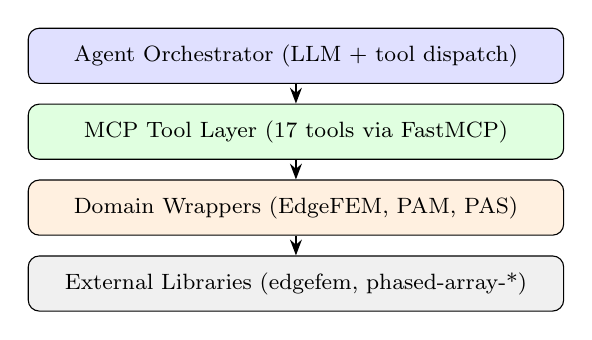
\begin{tikzpicture}[
  layer/.style={draw, rounded corners, minimum width=6.8cm,
    minimum height=0.7cm, align=center, font=\footnotesize},
  arr/.style={-{Stealth[length=2mm]}, thick},
  node distance=0.25cm
]
\node[layer, fill=blue!12] (agent) {Agent Orchestrator (LLM + tool dispatch)};
\node[layer, fill=green!12, below=of agent] (mcp) {MCP Tool Layer (17 tools via FastMCP)};
\node[layer, fill=orange!12, below=of mcp] (wrap) {Domain Wrappers (EdgeFEM, PAM, PAS)};
\node[layer, fill=gray!12, below=of wrap] (lib) {External Libraries (edgefem, phased-array-*)};
\draw[arr] (agent) -- (mcp);
\draw[arr] (mcp) -- (wrap);
\draw[arr] (wrap) -- (lib);
\end{tikzpicture}
\caption{Four-layer APAB pipeline architecture. The LLM agent
interacts only with the MCP layer; domain wrappers translate tool
calls to library-specific APIs.}
\label{fig:arch}
\end{figure}

% ======================================================================
\section{Case Study: 28\,GHz Patch Array}

We demonstrate the pipeline on an $8\times8$ rectangular microstrip
patch array on Rogers RO4003C ($\varepsilon_r = 3.55$,
$h = \SI{0.254}{\milli\meter}$, $\tan\delta = 0.0027$) with
half-wavelength spacing ($d = \SI{5.36}{\milli\meter}$).

\subsection{Unit-Cell Characterization}

EdgeFEM solves the unit cell with Floquet periodic boundary conditions
over \SIrange{26}{30}{\giga\hertz} (21~points). The Floquet reflection
phase transition locates the resonance at \SI{28.5}{\giga\hertz}.
An analytical cavity model using the Hammerstad effective permittivity
formula~\cite{hammerstad1975} and Bahl--Bhartia radiation
conductance~\cite{bahl1980} independently predicts \SI{28.4}{\giga\hertz}
---within 0.4\%. The analytical model yields a $-10$\,dB impedance
bandwidth of \SI{800}{\mega\hertz} (\SIrange{28.0}{28.8}{\giga\hertz}).

\subsection{Array Pattern}

A Taylor $\bar{n}$ taper~\cite{taylor1955} suppresses sidelobes below
$-\SI{25}{\deci\bel}$. At broadside, the tapered $8\times8$ array
achieves \SI{10.48}{dBi} directivity with \ang{16} half-power beamwidth.
Steering to $\theta_0 = \ang{15}$ incurs only \SI{0.02}{\deci\bel} scan
loss. Fig.~\ref{fig:results}(a) shows the E/H-plane cuts.

\subsection{Mutual Coupling}

A distance-dependent coupling model calibrated to published
measurements~\cite{pozar1994} populates the $64\times64$ S-matrix:
$-\SI{18}{\deci\bel}$ for adjacent elements, decaying to
$-\SI{24}{\deci\bel}$ at two lattice constants. The mean active
reflection coefficient is $\overline{|\Gamma|} = 0.265$, corresponding
to \SI{0.40}{\deci\bel} mismatch loss with no scan blindness
detected~\cite{pozar1984}. We note that this empirical model should be
validated against full-wave or measured S-parameters in future work.

\subsection{Link Budget}

For a 5G~NR downlink at \SI{200}{\meter} with \SI{400}{\mega\hertz}
bandwidth and \SI{0.1}{\watt} per element: total TX power =
\SI{6.4}{\watt}, array gain = \SI{23.0}{\deci\bel}, EIRP =
\SI{30.1}{dBW}, FSPL = \SI{107.4}{\deci\bel}, received SNR =
\SI{37.6}{\deci\bel}, and link margin = \SI{27.6}{\deci\bel} above the
\SI{10}{\deci\bel} threshold. Fig.~\ref{fig:results}(b) shows the
link-budget waterfall.

\subsection{Trade Study}

A 40-point Latin Hypercube Sampling~\cite{mckay1979} explores $N_x,
N_y \in [4, 16]$ and $P_\mathrm{elem} \in
[\SIrange{10}{500}{\milli\watt}]$. All designs exceed the SNR
requirement. EIRP spans \SIrange{22.3}{43.7}{dBW} with costs from
\$1,600 to \$25,600. The Pareto front reveals that a $9\times15$ array
at \SI{430}{\milli\watt}/element achieves 98\% of the maximum EIRP at
26\% lower cost than the largest design.

% ======================================================================
\section{Agent Validation}

To verify that the LLM agent produces correct results autonomously, we
ran the pipeline with Qwen~2.5 Coder (14B parameters) on a MacBook Pro
M3 with 32\,GB RAM. The agent:
\begin{itemize}
\item Correctly selected \texttt{pattern\_compute} and
  \texttt{system\_evaluate} from 17 available tools;
\item Self-corrected a missing parameter (\texttt{bandwidth\_hz}) after
  receiving a tool error, retrying successfully on the next turn;
\item Completed the full analysis in 4~LLM turns and 60~seconds wall
  time;
\item Produced a structured summary with directivity, link margin, and
  design recommendations consistent with the scripted pipeline results.
\end{itemize}

The complete tool-call trace is logged with timestamps for
reproducibility. The open-source APAB toolkit, all scripts, and
generated figures are available at~\cite{apab2026}.

% ======================================================================
\section{Conclusion}

We have demonstrated that an LLM agent can autonomously orchestrate
phased-array antenna analysis spanning unit-cell FEM simulation through
system-level trade studies. The 28\,GHz case study validates the
pipeline with 0.4\% FEM-analytical agreement, 27.6\,dB link margin, and
a 40-point trade study identifying cost-effective designs.

An autonomous optimization mode (\texttt{apab optimize}), inspired by
Karpathy's autoresearch framework~\cite{karpathy2026}, extends the
pipeline to iterative design exploration: the agent proposes parameter
changes, evaluates against a scalar metric with constraints, retains
improvements, and repeats---enabling overnight unattended optimization.

The current implementation uses an empirical mutual-coupling model;
future work will incorporate full-wave computed S-parameters and
measured element patterns. The APAB toolkit is extensible via plugin
entry points for additional LLM providers, EM solvers, and compute
backends.

\begin{figure}[!t]
\centering
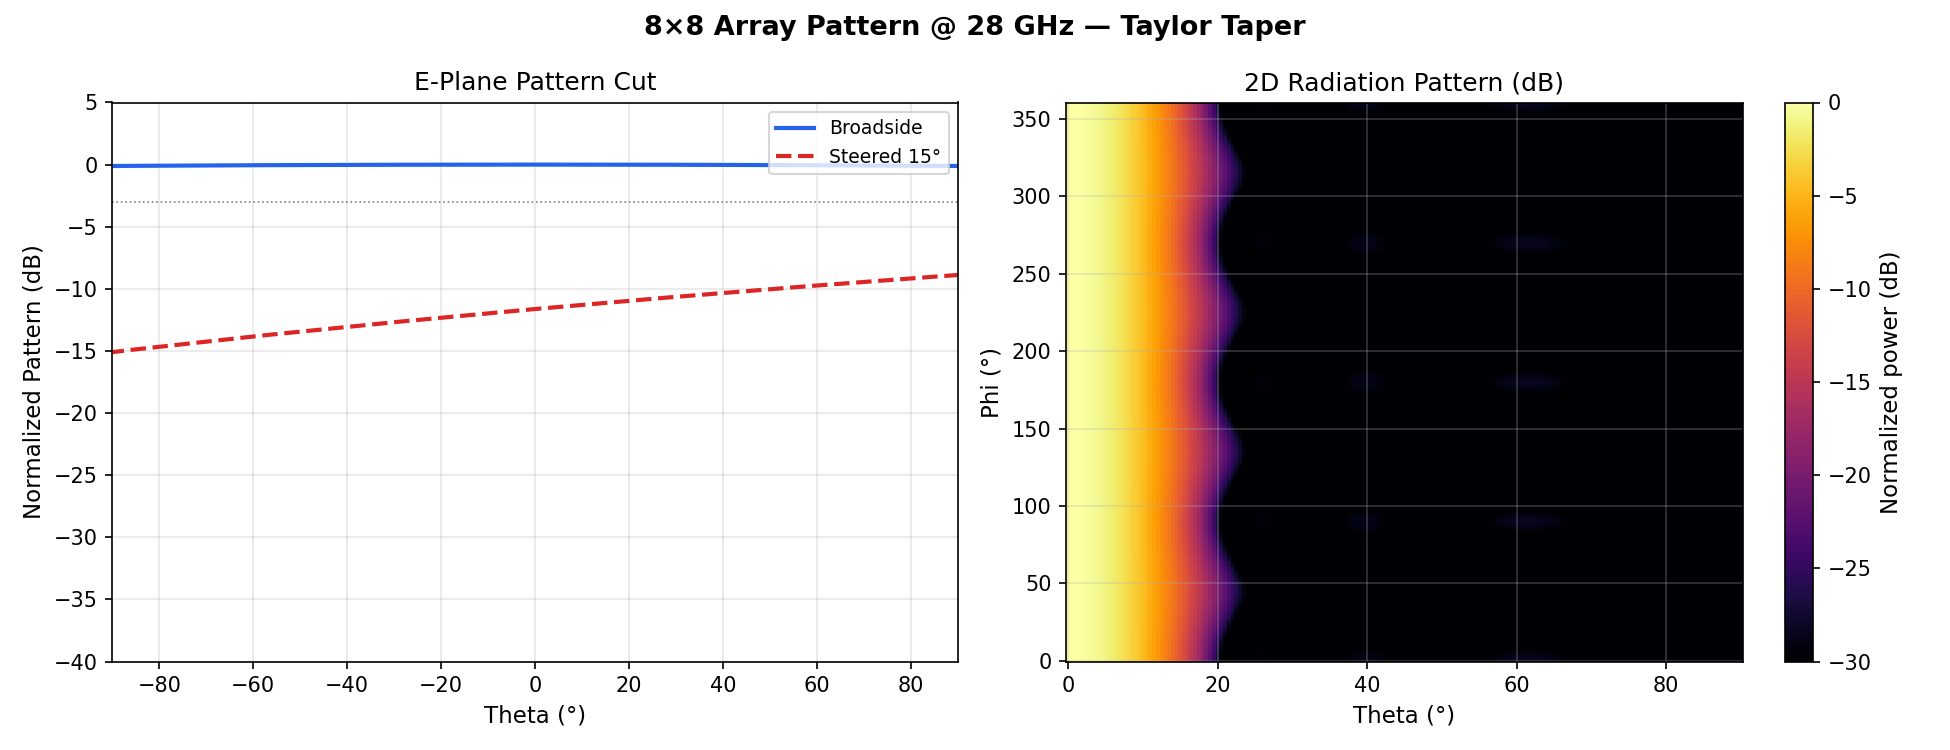
\includegraphics[width=\columnwidth]{fig2_array_pattern.png}
\vspace{-3mm}
\caption*{(a)}
\vspace{1mm}
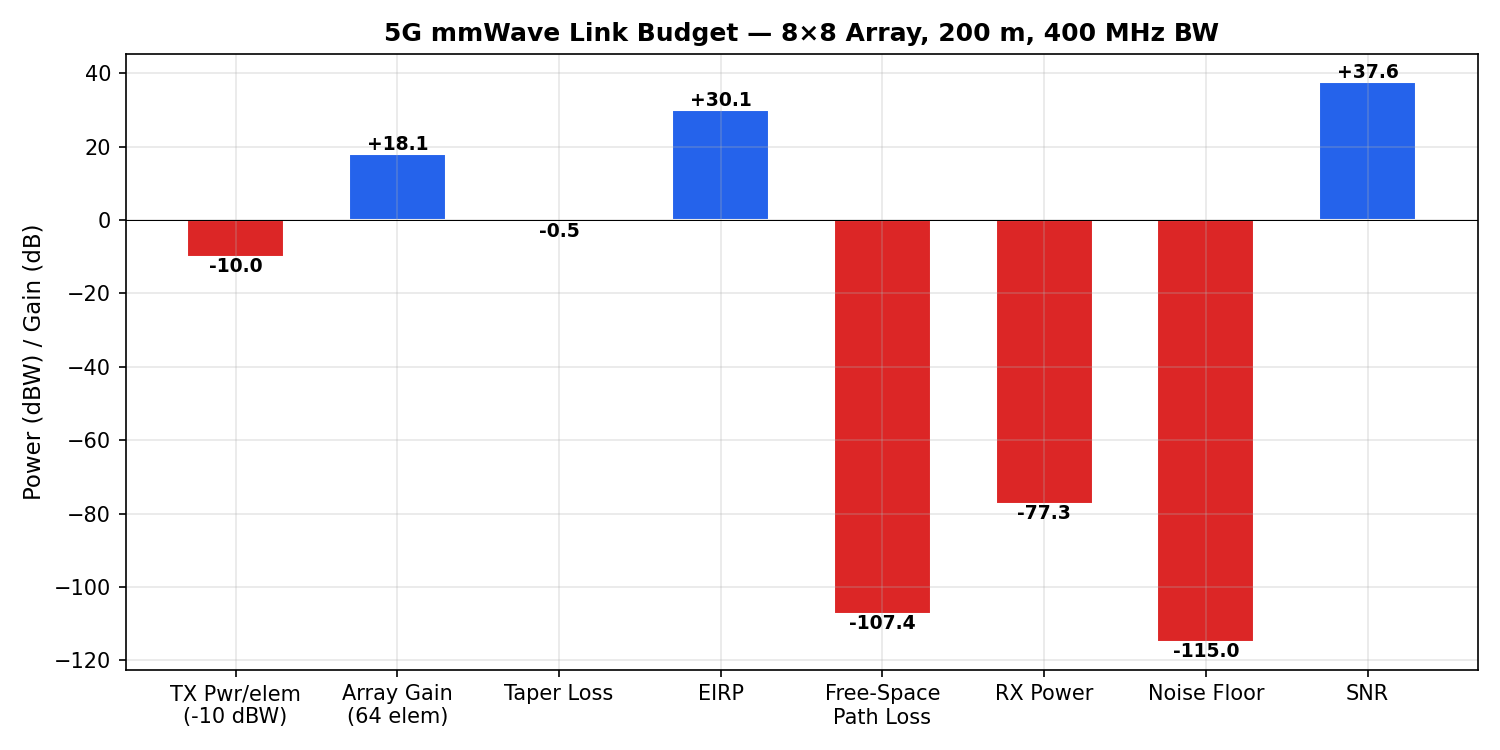
\includegraphics[width=\columnwidth]{fig4_link_budget.png}
\vspace{-3mm}
\caption*{(b)}
\caption{Case study results. (a)~Array radiation pattern: E-plane and
H-plane cuts, UV-space, and 3-D view for the $8\times8$ Taylor-tapered
array at 28\,GHz. (b)~Link-budget waterfall showing 27.6\,dB margin at
200\,m.}
\label{fig:results}
\end{figure}

% ======================================================================
\begin{thebibliography}{10}

\bibitem{balanis2016}
C.~A. Balanis, \emph{Antenna Theory: Analysis and Design}, 4th~ed.
Hoboken, NJ, USA: Wiley, 2016.

\bibitem{mailloux2017}
R.~J. Mailloux, \emph{Phased Array Antenna Handbook}, 3rd~ed.
Norwood, MA, USA: Artech House, 2017.

\bibitem{mcp2024}
Anthropic, ``Model Context Protocol specification,'' 2024. [Online].
Available: \url{https://modelcontextprotocol.io}

\bibitem{hammerstad1975}
E.~O. Hammerstad, ``Equations for microstrip circuit design,'' in
\emph{Proc. 5th Eur. Microw. Conf.}, Hamburg, Germany, Sep. 1975,
pp.~268--272.

\bibitem{bahl1980}
I.~J. Bahl and P.~Bhartia, \emph{Microstrip Antennas}.
Dedham, MA, USA: Artech House, 1980.

\bibitem{taylor1955}
T.~T. Taylor, ``Design of line-source antennas for narrow beamwidth
and low side lobes,'' \emph{IRE Trans. Antennas Propag.}, vol.~AP-3,
no.~1, pp.~16--28, Jan. 1955.

\bibitem{pozar1994}
D.~M. Pozar, ``The active element pattern,'' \emph{IEEE Trans.
Antennas Propag.}, vol.~42, no.~8, pp.~1176--1178, Aug. 1994.

\bibitem{pozar1984}
D.~M. Pozar and D.~H. Schaubert, ``Scan blindness in infinite phased
arrays of printed dipoles,'' \emph{IEEE Trans. Antennas Propag.},
vol.~32, no.~6, pp.~602--610, Jun. 1984.

\bibitem{mckay1979}
M.~D. McKay, R.~J. Beckman, and W.~J. Conover, ``A comparison of
three methods for selecting values of input variables in the analysis
of output from a computer code,'' \emph{Technometrics}, vol.~21,
no.~2, pp.~239--245, 1979.

\bibitem{karpathy2026}
A.~Karpathy, ``autoresearch --- Autonomous AI research,'' 2026.
[Online]. Available: \url{https://github.com/karpathy/autoresearch}

\bibitem{apab2026}
J.~A.~Hodge, ``APAB --- Agentic Phased Array Builder,'' 2026. [Online].
Available: \protect\url{https://github.com/jman4162/agentic-phased-array-builder}

\bibitem{edgefem2026}
J.~A.~Hodge, ``EdgeFEM --- 3-D finite-element electromagnetic solver,''
2026. [Online]. Available: \url{https://github.com/jman4162/EdgeFEM}

\end{thebibliography}

\end{document}
